\documentclass[../Práctica.root.tex]{subfiles}

\begin{document}

\section{Unidad 5}

\begin{enumerate}
  \item Un libro de física que se desliza sobre una mesa horizontal a \SI{1,10}{\meter\per\second} cae y llega al piso en \SI{0,350}{\second}. Ignore la resistencia del aire.

        \begin{center}
          \begin{tikzpicture}
            \draw (3,0) -- (8,0);
            \draw (0,0) rectangle (3,3);
            \draw (2,3) rectangle ++(1,.25);
            \draw[green,->] (3,3) parabola (6,0);
            \draw (6,0) node[above right, align=left]{$y_f=0$\\$t_f=\SI{0,350}{\second}$};
            \draw[red,->] (3,3.125) -- ++(1,0) node[right]{$V_x=\SI{1,10}{\meter\per\second}$};
          \end{tikzpicture}
        \end{center}

        \begin{enumerate}
          \item Calcule la altura de la mesa con respecto al piso.

                \[y_f=y_i+V_{yi}t_f+\frac{1}{2}a_y{t_f}^2\]
                \[0=y_i+\frac{1}{2}\cdot\SI{-9,80}{\meter\per\second\squared}\cdot(\SI{0,350}{\second})^2\]
                \[-y_i=\SI{-0,600}{\meter}\]
                \[y_i=\boxed{\SI{0,600}{\meter}}\]

          \item Calcule la distancia horizontal del borde de la mesa al punto donde cae el libro.

                \[x_f=x_i+V_xt_f\]
                \[x_f=\SI{1,10}{\meter\per\second}\cdot\SI{0,350}{\second}\]
                \[x_f=\boxed{\SI{0,385}{\meter}}\]
        \end{enumerate}

  \item Se lanza una piedra hacia arriba desde la parte superior de un edificio en un ángulo de \ang{30,0} con la horizontal y con una velocidad inicial de \SI{20,0}{\meter\per\second}. El punto de liberación está a \SI{45,0}{\meter} respecto de la superficie de la Tierra. Considere despreciable la resistencia del aire.

        \begin{center}
          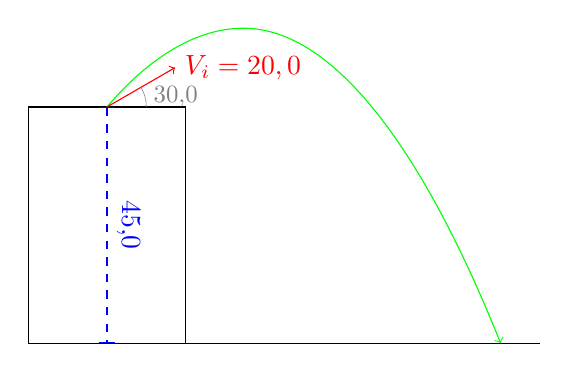
\begin{tikzpicture}
            \coordinate (a) at (1,3);
            \draw (2,0) -- (6.5,0);
            \draw (0,0) rectangle (2,3);
            \draw[green,->] (a) parabola bend ++(30:2) (6,0);
            \draw[red,->] (a) -- ++(30:1) node[right]{$V_i=\SI{20,0}{\meter\per\second}$};
            \draw[help lines] (a) ++(.5,0) arc (0:30:.5) node[pos=.5,right,scale=.9]{\ang{30,0}};
            \draw[dashed,blue,|-|] (a) -- (1,0) node[pos=.5,above,sloped]{\SI{45,0}{\meter}};
          \end{tikzpicture}
        \end{center}

        \begin{enumerate}
          \item ¿Cuánto tiempo le toma a la piedra golpear la superficie de la Tierra?

                \[V_{yi}=V_i\sin{\theta}=\SI{10,0}{\meter\per\second}\]

                \[y_f=y_i+V_{yi}t_f+\frac{1}{2}a_y{t_f}^2\]
                \[0=\SI{45,0}{\meter}+\SI{10,0}{\meter\per\second}t_f+\frac{1}{2}\cdot\SI{-9,80}{\meter\per\second\squared}{t_f}^2\]
                \[0=\SI{-4,90}{\meter\per\second\squared}{t_f}^2+\SI{10,0}{\meter\per\second}t_f+\SI{45,0}{\meter}\]

                \[\{t_1,t_2\}=\frac{-b\pm\sqrt{b^2-4ac}}{2a}\]
                \[\{t_1,t_2\}=\frac{\SI{-10,0}{\meter\per\second}\pm\sqrt{(\SI{10,0}{\meter\per\second})^2-4\cdot\SI{-4,90}{\meter\per\second\squared}\cdot\SI{45,0}{\meter}}}{2\cdot\SI{-4,90}{\meter\per\second\squared}}\]
                \[\{t_1,t_2\}=\frac{\SI{-10,0}{\meter\per\second}\pm\SI{31,3}{\meter\per\second}}{\SI{-9,80}{\meter\per\second\squared}}\]
                \[t_1=\SI{-2,17}{\second}, t_2=\SI{4,21}{\second}\]
                \[t_f=\boxed{\SI{4,21}{\second}}\]

          \item Determine la velocidad de la piedra en el impacto.

                \[V_x=V_i\cos{\theta}=\SI{17,3}{\meter\per\second}\]
                \[V_{yf}=V_{yi}+a_yt_f=\SI{-31,2}{\meter\per\second}\]
                \[V_f=\sqrt{{V_x}^2+{V_{yf}}^2}=\boxed{\SI{35,7}{\meter\per\second}}\]

          \item Encuentre el alcance horizontal de la piedra.

                \[x_f=x_i+V_xt_f=\boxed{\SI{72,8}{\meter}}\]
        \end{enumerate}

  \item Un CD gira desde el reposo hasta alcanzar una velocidad angular de \SI{31,4}{\radian\per\second} en un tiempo de \SI{0,892}{\second}.

        \begin{enumerate}
          \item ¿Cuál es la aceleración angular del CD suponiendo que ésta sea uniforme?

                \[\alpha=\frac{\Delta\omega}{\Delta t}=\frac{\SI{31,4}{\radian\per\second}}{\SI{0,892}{\second}}=\boxed{\SI{35,2}{\radian\per\second\squared}}\]

          \item ¿Qué ángulo ha recorrido el CD en su giro mientras alcanza su velocidad máxima?

                \[\theta_f=\theta_i+\omega_it_f+\frac{1}{2}\alpha{t_f}^2\]
                \[\theta_f=\frac{1}{2}\cdot\SI{35,2}{\radian\per\second\squared}\cdot(\SI{0,892}{\second})^2=\boxed{\SI{14,0}{\radian}}\]

          \item Si el radio del CD es \SI{4,45}{\cm}, encuentre la velocidad tangencial de un microbio que se mueve sobre el borde del CD cuando el tiempo es \SI{0,892}{\second}.

                \[V_{tf}=\omega_f r=\boxed{\SI{1,40}{\meter\per\second}}\]

          \item ¿Cuál es la magnitud de la aceleración tangencial del microbio en el tiempo dado?

                \[a_{tf}=\alpha_f r=\boxed{\SI{1,57}{\meter\per\second\squared}}\]
        \end{enumerate}

  \item Un río tiene una velocidad estable de \SI{0,500}{\meter\per\second}. Un estudiante nada en contra de la corriente una distancia de \SI{1,00}{\km} y nada de regreso al punto de partida.

        \begin{center}
          \begin{tikzpicture}
            \draw[green,->] (0,.33) -- ++(5,0) node[right]{$\alpha$};
            \draw[green,->] (5,-.33) -- ++(-5,0) node[left]{$\beta$};
            \draw[red,->] (5,1) -- ++(-5,0) node[pos=.5,above]{\SI{0,500}{\meter\per\second}};
            \draw[dashed,blue,|-|] (0,-1) -- ++(5,0) node[pos=.5,below]{\SI{1,00}{\km}};
          \end{tikzpicture}
        \end{center}

        \begin{enumerate}
          \item Si el estudiante puede nadar con una velocidad de \SI{1,20}{\meter\per\second} en aguas tranquilas, ¿cuánto tiempo le toma el viaje?

                \begin{multicols}{2}
                  \[x_{\alpha f}=V_{\alpha}t_{f\alpha}\]
                  \[\SI{1,00e3}{\meter}=\left(\SI{1,20}{\meter\per\second}-\SI{0,500}{\meter\per\second}\right)t_{\alpha f}\]
                  \[\SI{1,00e3}{\meter}=\SI{0,70}{\meter\per\second}t_{\alpha f}\]
                  \[t_{\alpha f}=\SI{1,43e3}{\second}\]

                  \[x_{\beta f}=V_{\beta}t_{f\beta}\]
                  \[\SI{1,00e3}{\meter}=\left(\SI{1,20}{\meter\per\second}+\SI{0,500}{\meter\per\second}\right)t_{\beta f}\]
                  \[\SI{1,00e3}{\meter}=\SI{1,70}{\meter\per\second}t_{\beta f}\]
                  \[t_{\beta f}=\SI{588}{\second}\]
                \end{multicols}

                \[t_f=t_{\alpha f}+t_{\beta f}=\SI{1,43e3}{\second}+\SI{588}{\second}=\boxed{\SI{2,02e3}{\second}}\]

          \item ¿Cuánto tiempo se requiere en aguas tranquilas para la misma distancia de nado?

                \[x_{\alpha f}=V_{\alpha}t_{f\alpha}\]
                \[\SI{1,00e3}{\meter}=\SI{1,20}{\meter\per\second}t_{\alpha f}\]
                \[t_{\alpha f}=\SI{833}{\second}\]
                \[t_{\beta f}=t_{\alpha f}\]
                \[t_f=2t_{\alpha f}=\boxed{\SI{1,67e3}{\second}}\]
        \end{enumerate}

  \item Un bombero que está a una distancia de \SI{50,0}{\meter} de un edificio en llamas dirige un chorro de agua desde el nivel del pavimento con un ángulo de \ang{30} respecto de la horizontal. Si la rapidez con que el chorro sale de la manguera es \SI{40,0}{\meter\per\second},

        \begin{center}
          \begin{tikzpicture}
            \draw (0,0) -- ++(5,0) -- ++(0,4);
            \coordinate (a) at (1,0);
            \draw[green,->] (a) to[out=60,in=190] (5,3);
            \draw[help lines] (a) ++(.5,0) arc (0:60:.5) node[pos=.5,right]{\ang{30}};
            \draw[red,->] (a) -- ++(60:1) node[left]{\SI{40,0}{\meter\per\second}};
            \draw[dashed,blue,|-|] (a) ++(0,-.2) -- ++(4,0) node[pos=.5,below]{\SI{50,0}{\meter}};
          \end{tikzpicture}
        \end{center}

        \begin{enumerate}
          \item ¿a qué altura el chorro golpeará al edificio?

                \[V_x=V_i\cos{\theta}=\SI{34,6}{\meter\per\second}\]

                \[x_f=x_i+V_xt_f\]
                \[\SI{50,0}{\meter}=\SI{34,6}{\meter\per\second}t_f\]
                \[t_f=\SI{1,45}{\second}\]

                \[V_{yi}=V_i\sin{\theta}=\SI{20,0}{\meter\per\second}\]

                \[y_f=y_i+V_{yi}t_f+\frac{1}{2}a_y{t_f}^2\]
                \[y_f=\SI{20,0}{\meter\per\second}\cdot\SI{1,45}{\second}+\frac{1}{2}\cdot\SI{-9,80}{\meter\per\second\squared}(\SI{1,45}{\second})^2\]
                \[y_f=\boxed{\SI{18,7}{\second}}\]

          \item ¿Refleja el dibujo el modo en que el chorro alcanza al edificio?

                \[V_y=V_{yi}+a_yt\]
                \[0=\SI{20}{\meter\per\second}-\SI{9,80}{\meter\per\second\squared}t_{max}\]
                \[t_{max}=\SI{2,04}{\second}\]
                \[t_{max}>t_f\]

                No. El chorro llega al edificio antes de llegar a su altura máxima.
        \end{enumerate}

  \item Un esquiador que se desliza por una rampa con una inclinación de \ang{30} llega al borde $A$ con cierta velocidad. Luego de \SI{1}{\second} de vuelo libre, retoma la pista en $B$ a \SI{4,33}{\meter} por delante del punto $A$.

        \begin{center}
          \begin{tikzpicture}
            \coordinate (a) at (0,4);
            \coordinate (b) at (3,0);
            \draw (a) node[above right]{$A$};
            \draw (a) -- ++(150:2);
            \draw[help lines, dashed] (a) -- ++(-2,0);
            \draw[help lines] (a) ++(150:1) arc (150:180:1) node[pos=.5,left]{\ang{30}};
            \draw[help lines, dashed] (a) -- ++(2,0);
            \draw[help lines, dashed] (a) -- ++(-30:2);
            \draw[help lines] (a) ++(-30:1) arc (-30:0:1) node[pos=.5,right]{\ang{30}};
            \draw[green, dashed, ->] (a) to[out=-30,in=100] (b);
            \draw (b) node[above right]{$B$};
            \draw[blue, dashed, |-|] (a |- 0,0) -- (b) node[pos=.5,below]{\SI{4,33}{\meter}};
          \end{tikzpicture}
        \end{center}

        \begin{enumerate}
          \item Hallar la velocidad que tiene en el punto A.

                \[x_f=x_i+V_xt_f\]
                \[\SI{4,33}{\meter}=V_x\cdot\SI{1,00}{\second}\]
                \[V_x=\SI{4,33}{\meter\per\second}\]

                \[V_x=V_i\cos{\theta}\]
                \[V_i=\frac{V_x}{\cos{\theta}}=\boxed{\SI{5,00}{\meter\per\second}}\]

          \item ¿Cuál es la altura entre los puntos A y B?

                \[V_{yi}=V_i\sin{\theta}=\SI{-2,50}{\meter\per\second}\]

                \[y_f=y_i+V_{yi}t_f+\frac{1}{2}a_y{t_f}^2\]
                \[0=y_i-\SI{2,50}{\meter\per\second}\cdot\SI{1,00}{\second}+\frac{1}{2}\cdot\SI{-9,80}{\meter\per\second\squared}(\SI{1,00}{\second})^2\]
                \[y_i=\boxed{\SI{7,40}{\meter}}\]

          \item ¿Qué velocidad final tendrá en B?

                \[V_{yf}=V_{yi}+a_yt_f=\SI{-12,3}{\meter\per\second}\]
                \[V_f=\sqrt{{V_x}^2+{V_{yf}}^2}=\boxed{\SI{13,0}{\meter\per\second}}\]
        \end{enumerate}

  \item Un automóvil tiene ruedas cuyo diámetro es de \SI{60,0}{\cm}, el mismo circula a velocidad constante de \SI{72,0}{\km\per\hour}.

        \begin{enumerate}
          \item ¿Cuál es el tiempo que tarda una de las ruedas en dar un giro completo?

                \[\Delta x=\pi d=\SI{188}{\cm}\]

                \[V=\frac{\Delta x}{\Delta t}\]
                \[\SI{72,0}{\km\per\hour}=\frac{\SI{188}{\cm}}{\Delta t}\]
                \[\Delta t=\frac{\SI{188}{\cm}}{\SI{72,0}{\km\per\hour}}\]
                \[\Delta t =
                  \frac{
                    \SI{188}{\cm} \cdot \frac{\SI{1}{\meter}}{
                                              \SI{100}{\cm}}
                  }{
                    \SI{72,0}{\km\per\hour} \cdot \SI{1000}{\meter\per\km} \cdot \frac{\SI{1}{\hour}}{
                                                                                        \SI{3600}{\second}}}=
                  \boxed{\SI{0,0940}{\second}}\]

          \item ¿Cuál es la velocidad angular de giro?

                \[\omega=\frac{\Delta\theta}{\Delta t}=\frac{\SI{2\pi}{\radian}}{\SI{0,0940}{\second}}=\boxed{\SI{66,8}{\radian\per\second}}\]
        \end{enumerate}
\end{enumerate}
\end{document}
